\chapter{Versatile Interface Adapter}
\label{chap_via}

The \jr\ includes a Western Design Center WDC65C22 versatile interface adapter or VIA. The VIA provides several useful features for I/O and timing:

\begin{itemize}
    \item Two independent I/O ports of eight parallel bits (PA, and PB).

    \item Four handshake control lines (CA1, CA2, CB1, and CB2)

    \item Programmable serial register for serial I/O operations

    \item Two independent timer counters
\end{itemize}

On the \jr, the VIA is connected to header which is compatible with the keyboard header on the Commodore VIC-20 and C-64. This means that a Commodore compatible keyboard could be connected to the \jr\ and used for keyboard input with appropriate programming. The VIA also provides access to the two Atari-style joystick ports. The pins could also be used for general purpose I/O, although the voltage levels are for 3.3 volt logic instead of the 5 volt logic used in older 8-bit machines. The internal circuitry of the VIA's port A and port B I/O pins is shown in figure~\ref{fig:via_pin}.

\begin{note}
    While the \fjr\ has a single VIA, the \fk\ has two VIA chips. The second VIA chip is located at 0xDB00. The purpose of this second VIA is to manage the built-in keyboard of the \fk, while the first VIA is used solely for the joystick. On the \fjr, the single VIA handles either the joystick or the keyboard. See page \pageref{sec_f256k_kbd} for a more complete description of the keyboard.
\end{note}

A complete description of the VIA would be rather long, so this guide will merely list out the register addresses and provide a quick break-down on the register functions. For a complete description, please see the data sheet from Western Design Center. See table~\ref{tab:via_reg} for a listing of all the VIA registers.

\begin{table}[ht]
    \begin{center}
        \begin{tabular}{|c|c|c|l|} \hline
            Address & R/W & Name & Purpose \\\hline\hline
            \verb+0xDC00+ & R/W & IORB & Port B data \\\hline
            \verb+0xDC01+ & R/W & IORA & Port A data \\\hline
            \verb+0xDC02+ & R/W & DDRB & Port B Data Direction Register \\\hline
            \verb+0xDC03+ & R/W & DDRA & Port A Data Direction Register \\\hline
            \verb+0xDC04+ & R/W & T1C\_L & Timer 1 Counter Low \\\hline
            \verb+0xDC05+ & R/W & T1C\_H & Timer 1 Counter High \\\hline
            \verb+0xDC06+ & R/W & T1L\_L & Timer 1 Latch Low \\\hline
            \verb+0xDC07+ & R/W & T1L\_H & Timer 1 Latch High \\\hline
            \verb+0xDC08+ & R/W & T2C\_L & Timer 2 Counter Low \\\hline
            \verb+0xDC09+ & R/W & T2C\_H & Timer 2 Counter High \\\hline
            \verb+0xDC0A+ & R/W & SDR & Serial Data Register \\\hline
            \verb+0xDC0B+ & R/W & ACR & Auxiliary Control Register \\\hline
            \verb+0xDC0C+ & R/W & PCR & Peripheral Control Register \\\hline
            \verb+0xDC0D+ & R/W & IFR & Interrupt Flag Register \\\hline
            \verb+0xDC0E+ & R/W & IER & Interrupt Enable Register \\\hline
            \verb+0xDC0F+ & R/W & IORA2 & Port A data (no handshake) \\\hline
        \end{tabular}
    \end{center}
    \caption{VIA Registers}
    \label{tab:via_reg}
\end{table}

\begin{table}[ht]
    \begin{center}
        \begin{tabular}{|c|c|c|c|c|c|c|c|c|} \hline
            Name & 7 & 6 & 5 & 4 & 3 & 2 & 1 & 0 \\\hline\hline
            ACR & \multicolumn{2}{|c|}{T1\_CTRL} & T2\_CTRL & \multicolumn{3}{|c|}{SR\_CTRL} & PBL\_EN & PAL\_EN \\\hline
            PCR & \multicolumn{3}{|c|}{CB2\_CTRL} & CB1\_CTRL & \multicolumn{3}{|c|}{CA2\_CTRL} & CA1\_CTRL \\\hline
            IFR & IRQF & T1F & T2F & CB1F & CB2F & SRF & CA1F & CA2F \\\hline
            IER & SET & T1E & T2E & CB1E & CB2E & SRE & CA1E & CA2E \\\hline
        \end{tabular}
    \end{center}
    \caption{VIA Control Registers}
    \label{tab:via_ctrl_reg}
\end{table}

\begin{description}
    \item[IORA] Input/Output Register for Port A. The eight bits correspond to the eight pins on port A.

    \item[DDRA] Data Direction Register for Port A. Each bit configures the corresponding pin to be input (0) or output (1).

    \item[IORB] Input/Output Register for Port B. The eight bits correspond to the eight pins on port B.

    \item[DDRB] Data Direction Register for Port B. Each bit configures the corresponding pin to be input (0) or output (1).

    \item[T1C\_L, T1C\_H] Timer 1 counter value

    \item[T1L\_L, T1L\_H] Timer 1 latch

    \item[T2C\_L, T2C\_H] Timer 2 counter value

    \item[SDR] is the shift register. Serial input may be read here, or data may be written here to be shifted out.

    \item[ACR] Auxiliary Control Register. Contains fields to control the function of timer 1, timer 2, the shift register, and how Port A and Port B latch data. See table~\ref{tab:via_ctrl_reg} for details.

    \item[PCR] Peripheral Control Register. Contains fields to control how the CA1, CA2, CB1, and CB2 handshake pins are used. See table~\ref{tab:via_ctrl_reg} for details.

    \item[IFR] Interrupt Flag Register. Contains flags indicating which condition triggered an interrupt request. Possible conditions are timer 1, timer 2, CB1, CB2, CA1, CA2, and shift register complete. See table~\ref{tab:via_ctrl_reg} for details.

    \item[IER] Interrupt Enable Register. Contains flags to enable or disable interrupts based on the different possible conditions. See table~\ref{tab:via_ctrl_reg} for details.

    \item[IORA2] Same as IOPA except that the built-in handshaking capability is not used.

\end{description}

\begin{figure}[ht]
    \begin{center}
        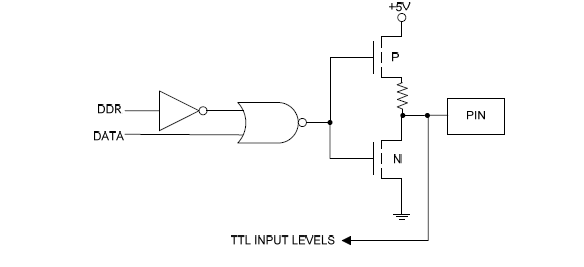
\includegraphics[scale=0.65]{images/via_pin_drivers.png}
    \end{center}
    \caption{VIA Pin Internal Circuitry}
    \label{fig:via_pin}
\end{figure}